\documentclass[english, xcolor=dvipsnames, aspectratio=169]{beamer}
\setbeamertemplate{navigation symbols}{}

\usepackage[english]{babel}
\usepackage{amsmath,amssymb,booktabs,graphicx}
\usepackage{tikz}
\usetikzlibrary{arrows.meta,positioning}

\graphicspath{{png_figures/}}

\definecolor{ecgred}{HTML}{A33B2E}
\definecolor{ecgteal}{HTML}{2F6F73}
\setbeamercolor{palette primary}{bg=ecgred,fg=white}
\setbeamercolor{palette secondary}{bg=ecgred,fg=white}
\setbeamercolor{palette tertiary}{bg=ecgred,fg=white}
\setbeamercolor{palette quaternary}{bg=ecgred,fg=white}
\setbeamercolor{structure}{fg=ecgred}
\setbeamercolor{block title}{bg=ecgred,fg=white}
\setbeamercolor{block body}{bg=black!5,fg=black}

\setbeamertemplate{footline}{
  \leavevmode
  \hbox{
  \begin{beamercolorbox}[wd=.33\paperwidth,ht=2.6ex,dp=1ex,center]{palette quaternary}ECG RMT Analysis\end{beamercolorbox}
  \begin{beamercolorbox}[wd=.33\paperwidth,ht=2.6ex,dp=1ex,center]{palette quaternary}PTB-XL\end{beamercolorbox}
  \begin{beamercolorbox}[wd=.33\paperwidth,ht=2.6ex,dp=1ex,center]{palette quaternary}\insertframenumber{} / \inserttotalframenumber\end{beamercolorbox}}
}

\title{High-Dimensional Arrhythmia Classification from Raw ECG Time Series}
\subtitle{PTB-XL preprocessing, model selection, spectral analysis, and RMT diagnostics}
\author{ECG RMT Analysis}
\date{May 2026}

\begin{document}

\begin{frame}
\titlepage
\end{frame}

\begin{frame}{Project Goal}
\begin{block}{Task}
Build a complete applied-ML pipeline for binary ECG screening from PTB-XL raw waveform records, then analyze fitted model behavior in the high-dimensional feature regime.
\end{block}
\begin{itemize}
\item Input: ten-second, twelve-lead ECG waveform plus metadata.
\item Target: normal versus diagnostic abnormality from SCP diagnostic superclasses.
\item Evaluation: official PTB-XL folds.
\item RMT role: diagnostic layer, not a classifier.
\end{itemize}
\end{frame}

\begin{frame}{Dataset and Labels}
\begin{columns}[T,totalwidth=\textwidth]
\begin{column}{0.48\textwidth}
\begin{block}{PTB-XL}
\begin{itemize}
\item 21,799 metadata rows.
\item WFDB waveform files.
\item 100 Hz and 500 Hz records.
\item SCP-ECG statement dictionaries.
\end{itemize}
\end{block}
\end{column}
\begin{column}{0.48\textwidth}
\begin{block}{Supervised table}
\begin{center}
\begin{tabular}{lr}
\toprule
Quantity & Count \\
\midrule
Labeled records & 21,388 \\
Normal & 9,069 \\
Diagnostic abnormality & 12,319 \\
\bottomrule
\end{tabular}
\end{center}
\end{block}
\end{column}
\end{columns}
\end{frame}

\begin{frame}{Pipeline}
\begin{center}
\resizebox{\linewidth}{!}{%
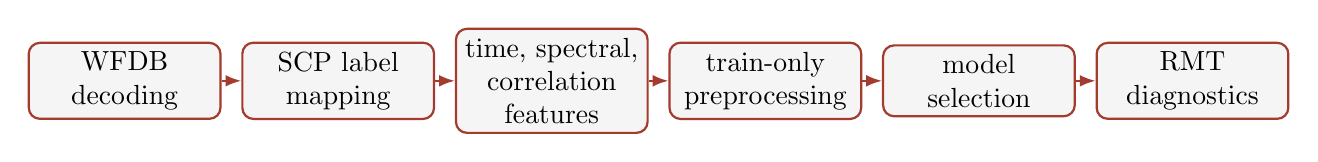
\begin{tikzpicture}[
  node distance=0.25cm,
  box/.style={draw=ecgred, rounded corners, thick, align=center, minimum height=0.8cm, text width=2.2cm, fill=black!4},
  arr/.style={-{Latex[length=2mm]}, thick, ecgred}
]
\node[box] (wfdb) {WFDB\\decoding};
\node[box, right=of wfdb] (labels) {SCP label\\mapping};
\node[box, right=of labels] (features) {time, spectral,\\correlation features};
\node[box, right=of features] (prep) {train-only\\preprocessing};
\node[box, right=of prep] (models) {model\\selection};
\node[box, right=of models] (rmt) {RMT\\diagnostics};
\draw[arr] (wfdb) -- (labels);
\draw[arr] (labels) -- (features);
\draw[arr] (features) -- (prep);
\draw[arr] (prep) -- (models);
\draw[arr] (models) -- (rmt);
\end{tikzpicture}
}
\end{center}
\begin{block}{Reproducibility point}
Preprocessing statistics are fit only on training folds; validation and test folds are never used for imputation or scaling.
\end{block}
\end{frame}

\begin{frame}{Feature Map}
\[
z_i=\phi(r_i,q_i)\in\mathbb{R}^{523},
\qquad
x_i=g(z_i)\in\mathbb{R}^{594}.
\]
\begin{columns}[T,totalwidth=\textwidth]
\begin{column}{0.32\textwidth}
\begin{block}{Time-domain}
moments, quantiles, RMS, energy, derivatives, zero crossings
\end{block}
\end{column}
\begin{column}{0.32\textwidth}
\begin{block}{Frequency-domain}
FFT power, centroid, entropy, dominant frequency, roll-off, band powers
\end{block}
\end{column}
\begin{column}{0.32\textwidth}
\begin{block}{Metadata and leads}
age, sex, height, weight, site, device, and pairwise lead correlations
\end{block}
\end{column}
\end{columns}
\end{frame}

\begin{frame}{Preprocessing Findings}
\centering
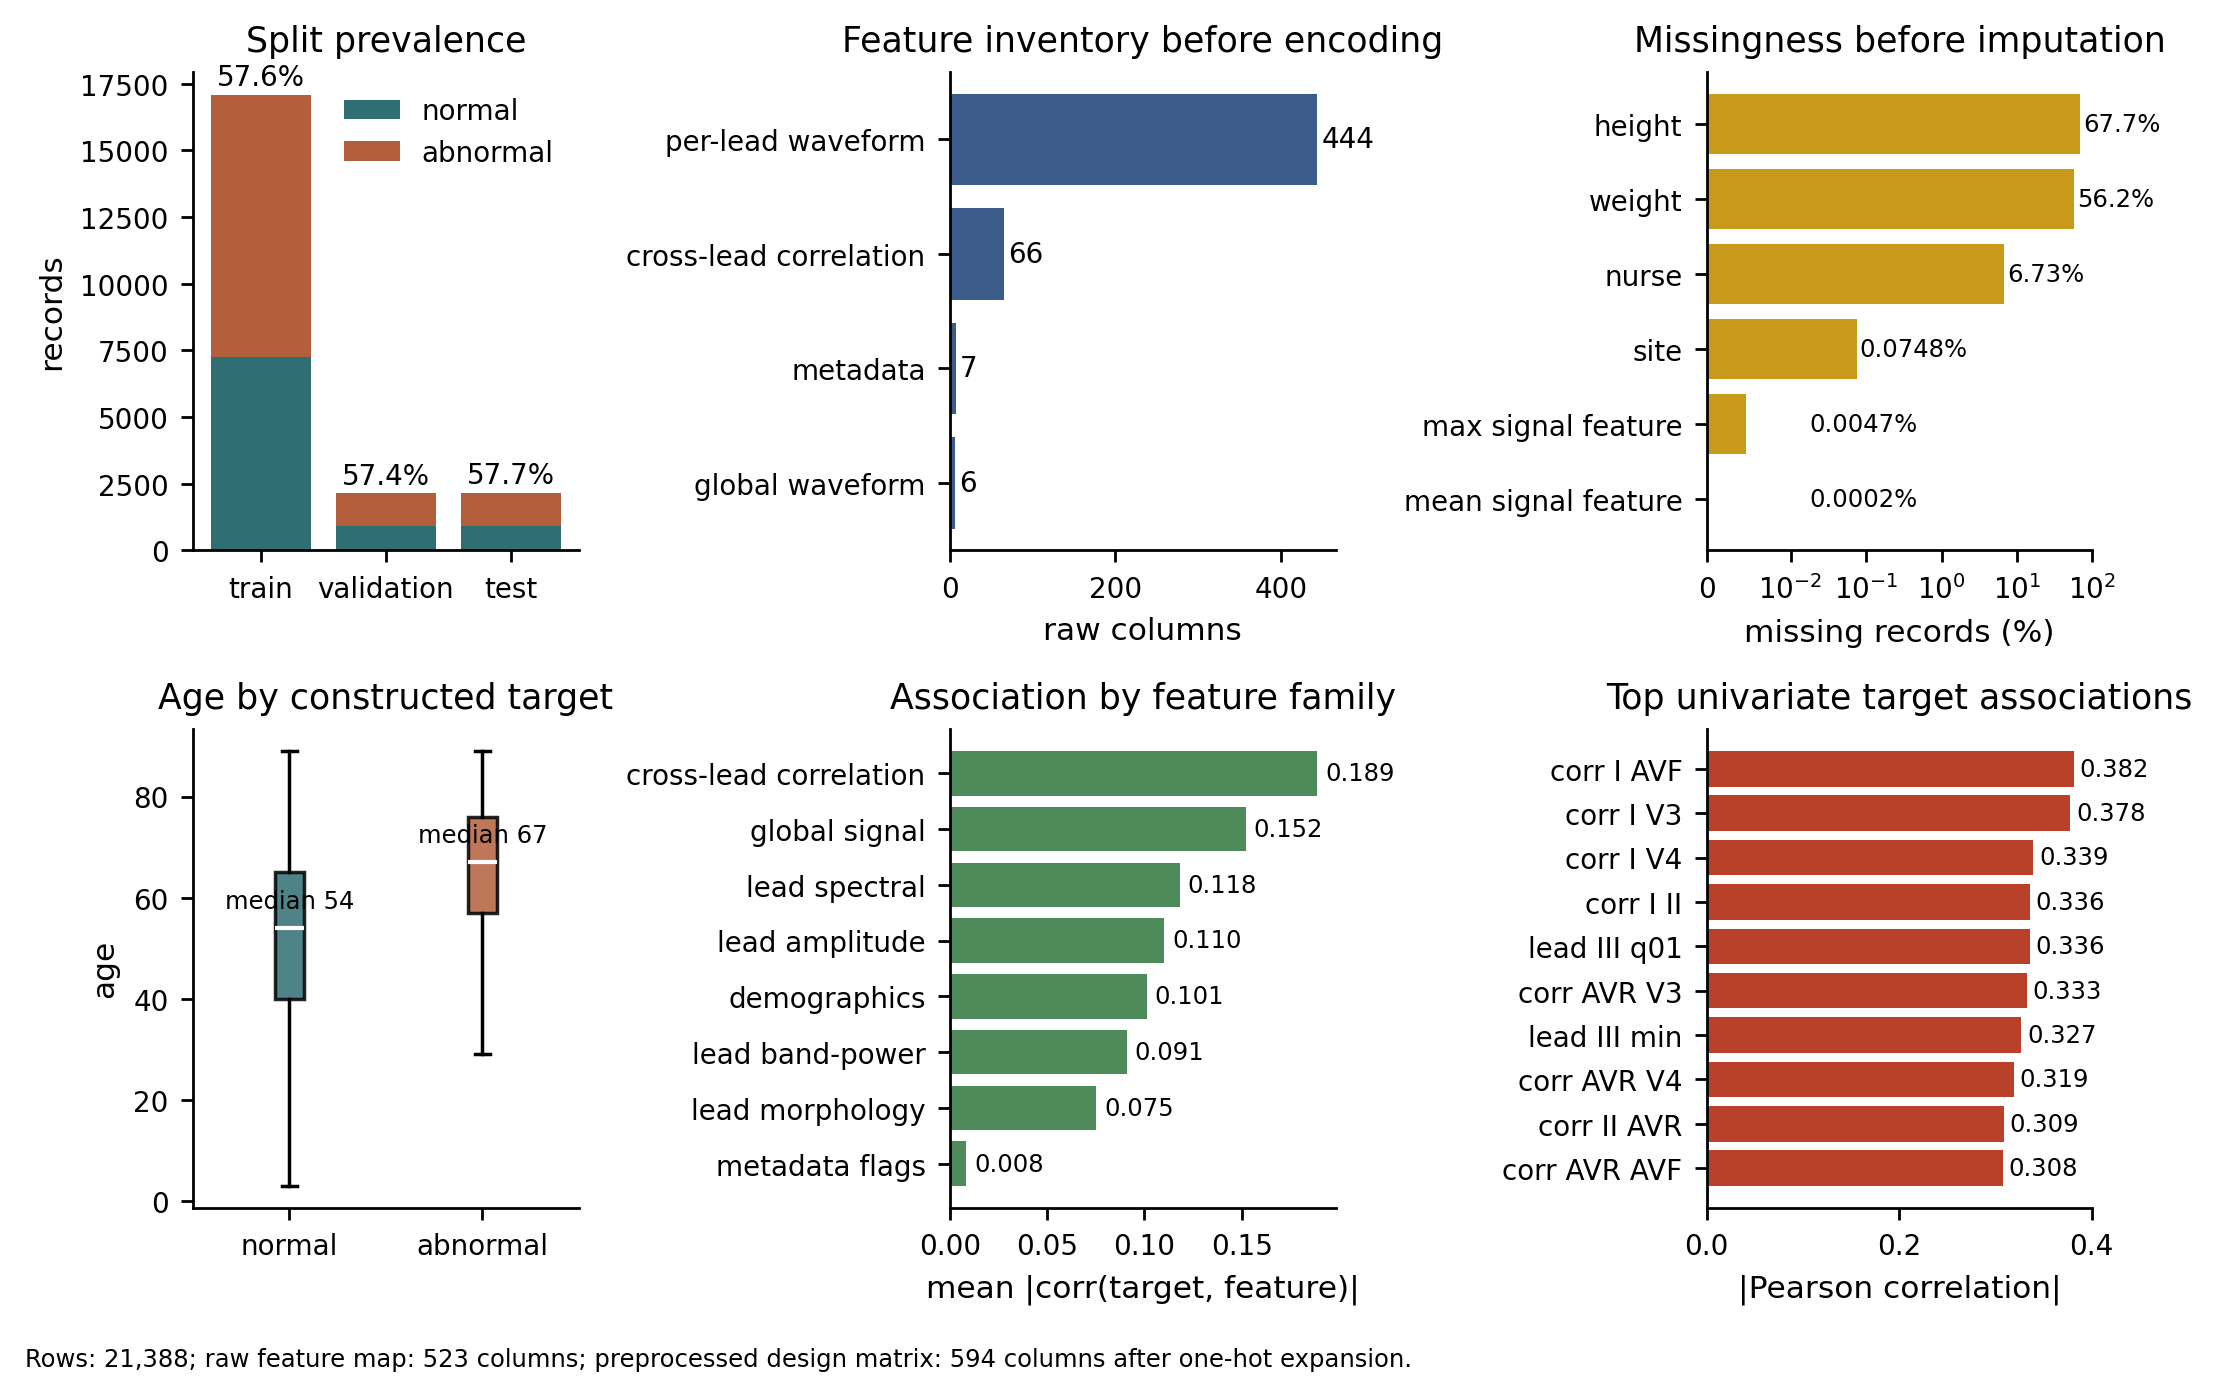
\includegraphics[height=0.76\paperheight,keepaspectratio]{paper_preprocessing_findings.png}
\end{frame}

\begin{frame}{Model Families}
\begin{center}
\small
\begin{tabular}{lp{8.8cm}}
\toprule
Model & Role \\
\midrule
Logistic regression & Regularized linear baseline. \\
SGD linear & Fast high-dimensional margin model. \\
Random forest & Bagged nonlinear tree ensemble. \\
Extra trees & Higher-randomness tree ensemble. \\
Histogram gradient boosting & Strong CPU boosting baseline. \\
XGBoost & Regularized boosted trees with GPU support. \\
\bottomrule
\end{tabular}
\end{center}
\end{frame}

\begin{frame}{Final Test Metrics}
\begin{center}
\scriptsize
\begin{tabular}{lrrrrrr}
\toprule
Model & Acc. & Bal. acc. & Prec. & Recall & F1 & ROC-AUC \\
\midrule
Logistic regression & 0.7938 & 0.8044 & 0.8877 & 0.7360 & 0.8047 & 0.8924 \\
SGD linear & 0.7271 & 0.7307 & 0.7973 & 0.7071 & 0.7495 & 0.7307 \\
Random forest & 0.8100 & 0.8115 & 0.8597 & 0.8018 & 0.8297 & 0.9001 \\
Extra trees & 0.8021 & 0.8072 & 0.8686 & 0.7745 & 0.8188 & 0.8909 \\
Hist. gradient boosting & 0.8202 & 0.8231 & 0.8743 & 0.8042 & 0.8378 & 0.9089 \\
XGBoost & 0.8151 & 0.8183 & 0.8712 & 0.7978 & 0.8328 & 0.9097 \\
\bottomrule
\end{tabular}
\end{center}
\begin{block}{Result}
XGBoost has the highest ROC-AUC; histogram gradient boosting has the highest F1.
\end{block}
\end{frame}

\begin{frame}{Model Comparison and RMT Summary}
\centering
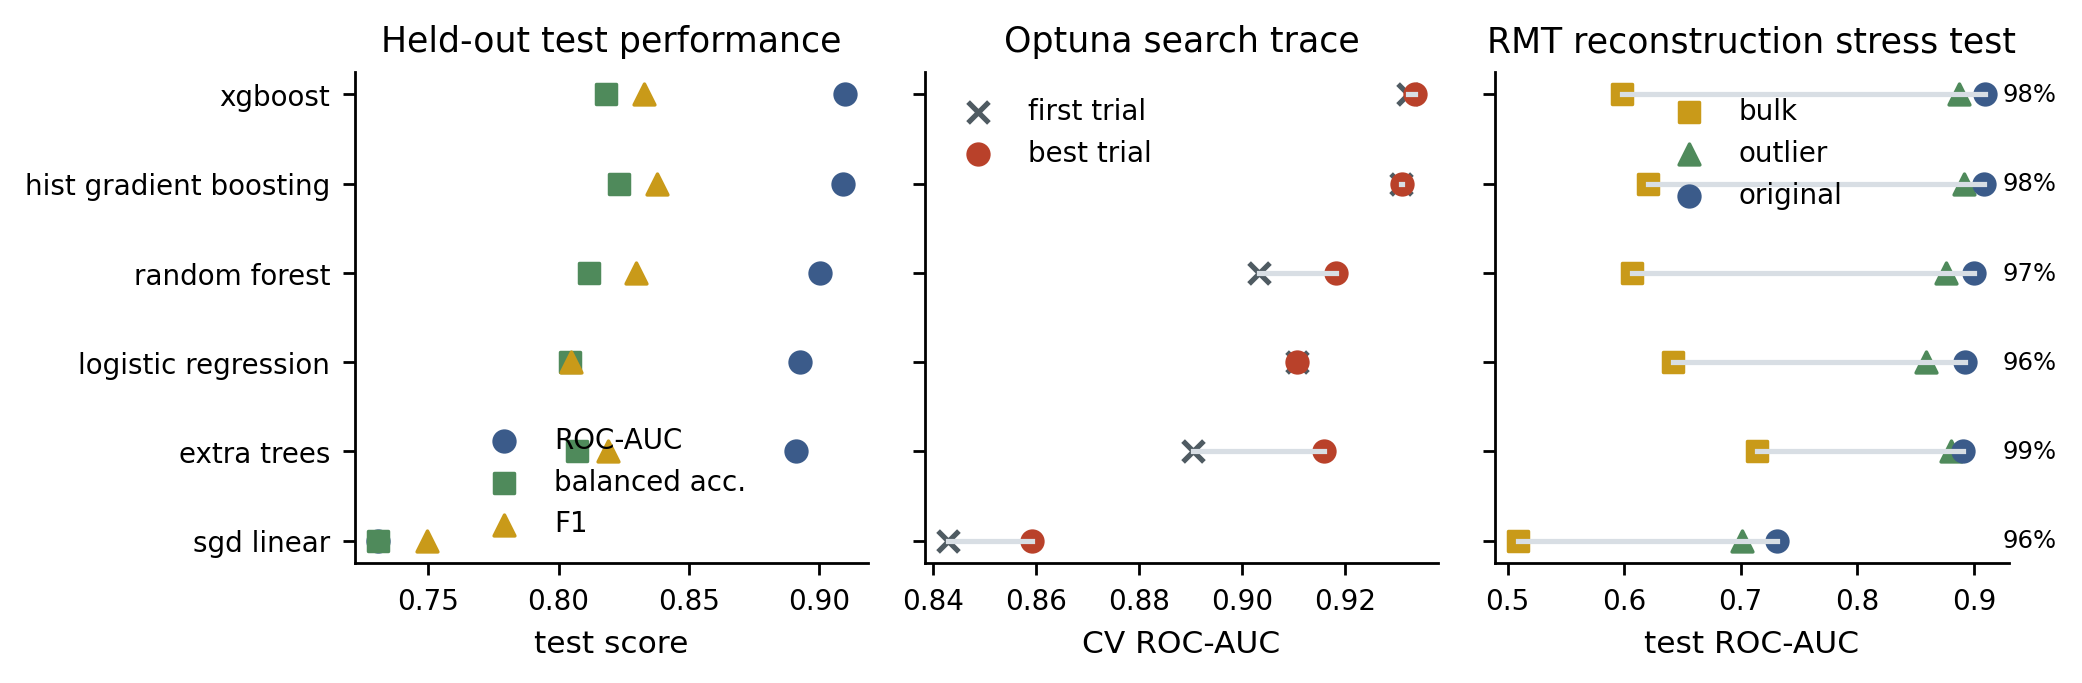
\includegraphics[width=0.96\linewidth]{paper_model_rmt_summary.png}
\end{frame}

\begin{frame}{Why RMT?}
\begin{block}{Marchenko--Pastur reference}
For standardized white-noise features with aspect ratio \(\gamma=p/n\),
\[
\lambda_\pm=(1\pm\sqrt{\gamma})^2.
\]
\end{block}
\begin{itemize}
\item Eigenvalues inside the support form the empirical bulk.
\item Eigenvalues above the upper edge are structured outliers.
\item The diagnostic checks whether trained models rely on outliers or bulk.
\end{itemize}
\end{frame}

\begin{frame}{Dataset Covariance Spectrum}
\centering
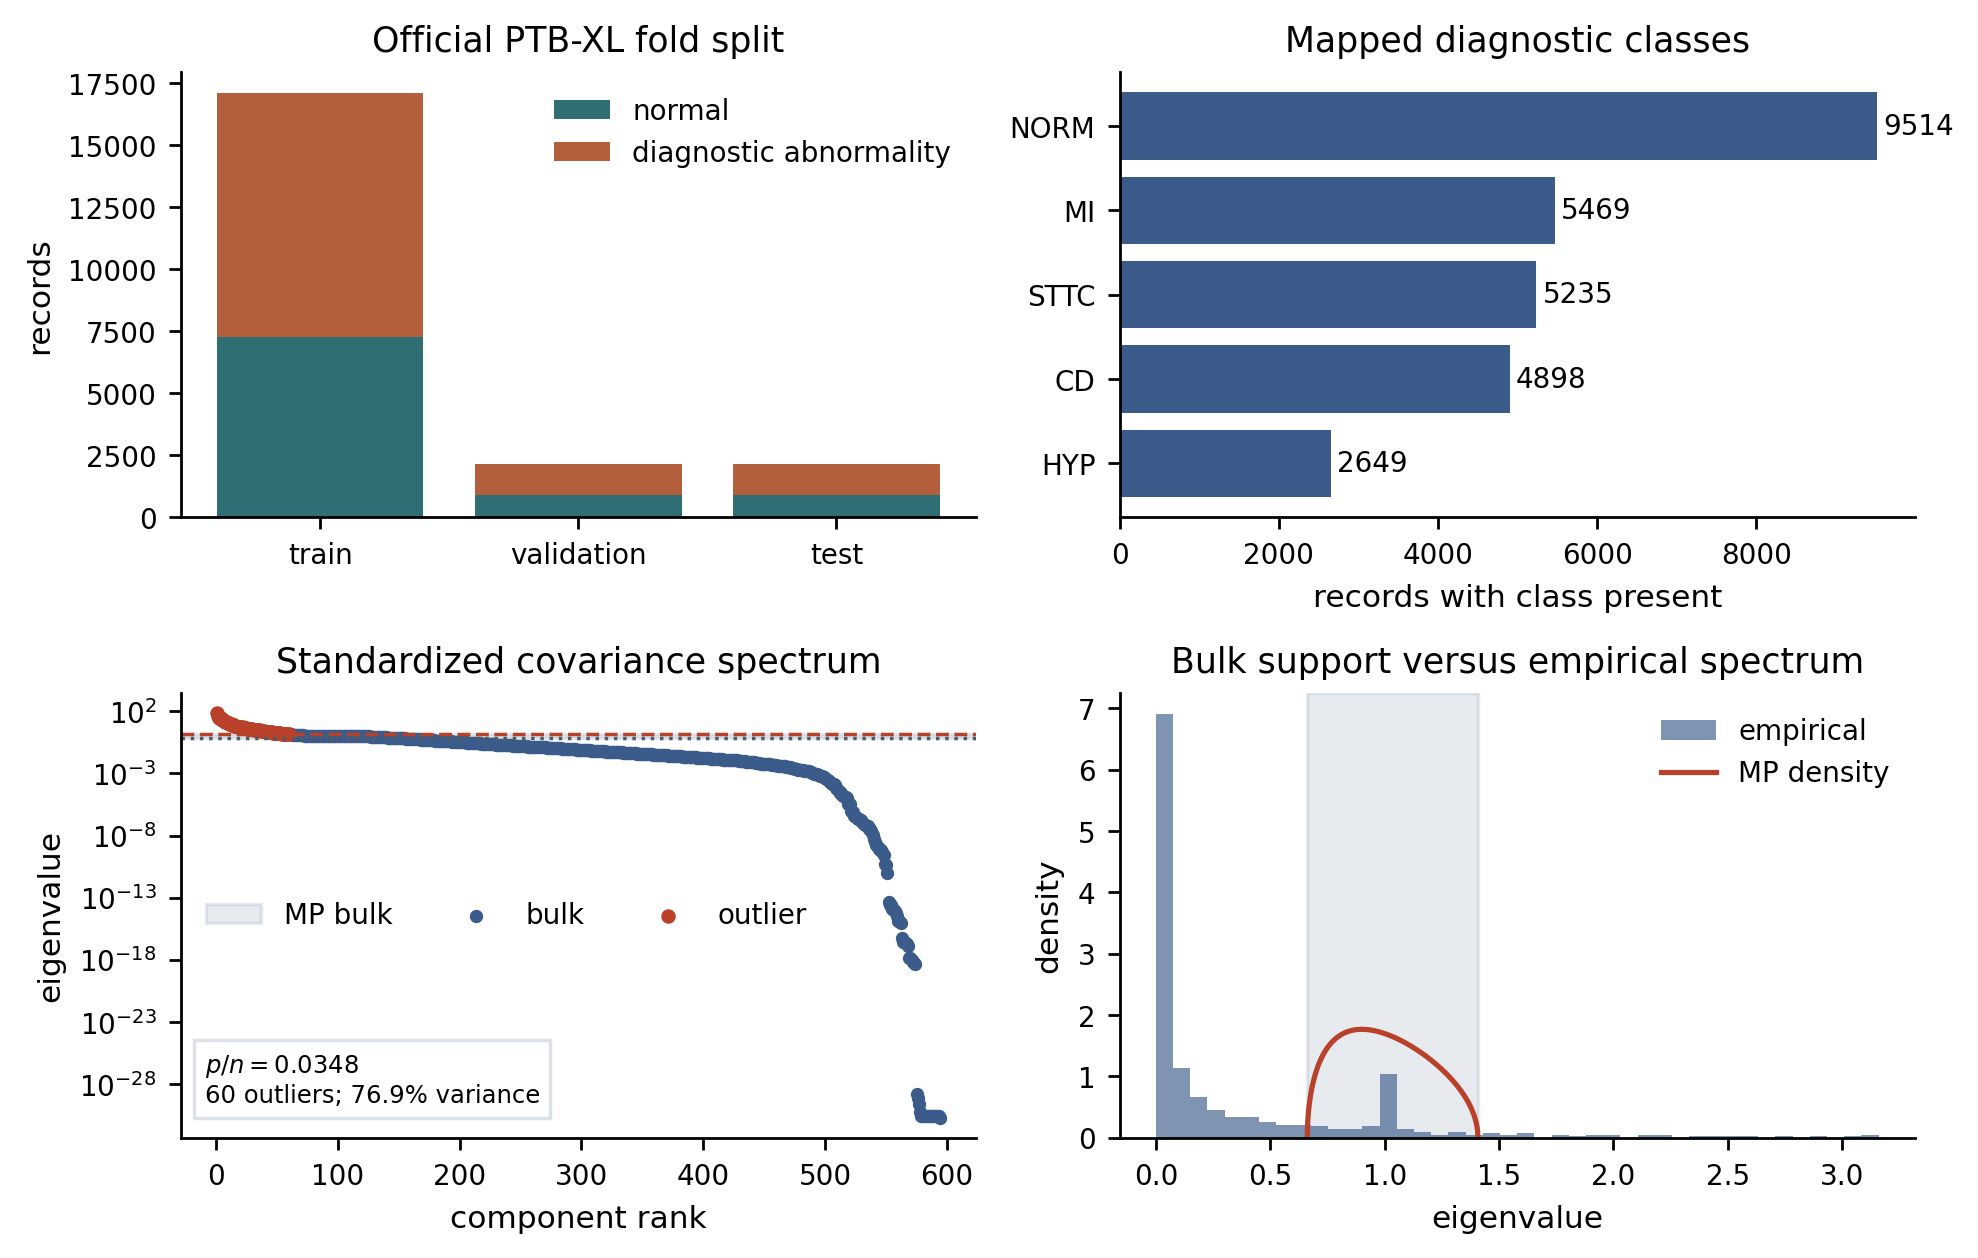
\includegraphics[height=0.76\paperheight,keepaspectratio]{paper_dataset_spectrum.png}
\end{frame}

\begin{frame}{RMT Findings}
\begin{itemize}
\item \(p/n=0.0348\).
\item MP support is \([0.662,1.408]\).
\item 60 components lie above the upper edge.
\item Outlier components explain 76.9\% of standardized variance.
\item MP-outlier reconstructions preserve most model discrimination.
\item MP-bulk reconstructions are weaker but not completely uninformative.
\end{itemize}
\end{frame}

\begin{frame}{Filtering Experiment}
\centering
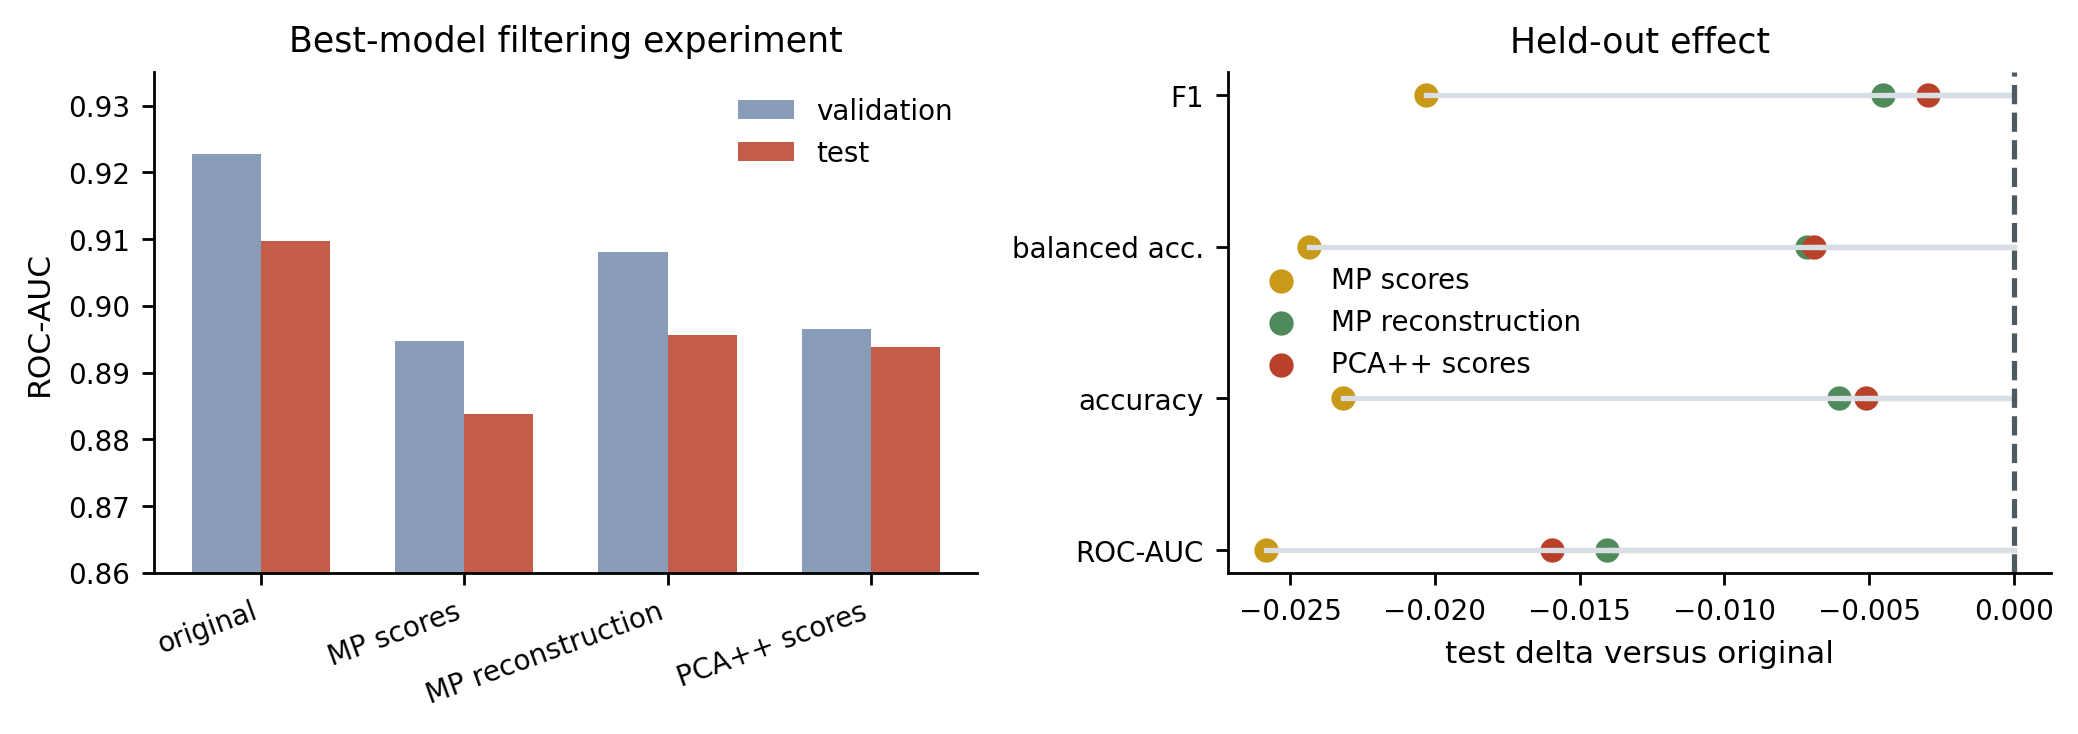
\includegraphics[width=0.96\linewidth]{paper_rmt_filtering_experiment.png}
\end{frame}

\begin{frame}{Main Takeaways}
\begin{enumerate}
\item Raw PTB-XL waveforms can be turned into a reproducible binary ECG screening pipeline.
\item Boosted trees produce the strongest held-out results in this feature space.
\item Metadata missingness and cohort age shift are important preprocessing findings.
\item The covariance spectrum has a small dominant outlier subspace.
\item RMT explains model behavior better than it improves the classifier here.
\end{enumerate}
\end{frame}

\begin{frame}[plain]
\centering
\vfill
{\Huge Questions?}

\vspace{0.8cm}
Raw ECG decoding \(\rightarrow\) feature engineering \(\rightarrow\) model selection \(\rightarrow\) spectral diagnostics.
\vfill
\end{frame}

\end{document}
